\documentclass{article}

% packages and configurations
\usepackage{hyperref}
\usepackage{animate} % needed for animations and videos
\usepackage{bm} % bold font in equation environments
\usepackage[utf8]{inputenc}	% für Umlaute ect.
\usepackage{fancyhdr} % für header
\usepackage{lastpage} % für footer
\usepackage{extramarks} % für header und footer
\usepackage{amsthm} % math stuff
\usepackage{amsmath} % math stuff
\usepackage{amssymb} % math stuff
\usepackage{color}
\usepackage[procnames]{listings} % code listings
\usepackage{graphicx} % für graphics
\usepackage[toc]{glossaries} % Glossar
\usepackage{color}
\usepackage{tikz}
\usepackage[absolute,overlay]{textpos} %to translate graphics through space
\usepackage{soul}
\usepackage{xcolor}
\usepackage{textpos}
\usepackage{caption}
\usepackage{parcolumns}
\usepackage{enumerate}
\usepackage[ngerman]{babel} % Umlaute
\usepackage[T1]{fontenc}    % this is needed for correct output of umlauts in pd
\usepackage[section]{placeins} %forces placeins to stay in section
\usepackage{datetime} % custom dates
\usepackage{afterpage}
\usepackage[section]{placeins}

\definecolor{keywords}{RGB}{255,0,90}
\definecolor{comments}{RGB}{0,0,113}
\definecolor{red}{RGB}{160,0,0}
\definecolor{green}{RGB}{0,150,0}

\lstset{language=Python, 
	basicstyle=\ttfamily\small, 
	keywordstyle=\color{keywords},
	commentstyle=\color{comments},
	stringstyle=\color{red},
	showstringspaces=false,
	identifierstyle=\color{green},
	procnamekeys={def,class}}

\title{Bringing together visual analytics and probabilistic programming languages}
\author{Jonas Aaron Gütter  \\
	Friedrich Schiller Universität Jena  \\
    Matrikelnr 152127 \\
    Prof.Dr. Joachim Giesen \\
    M. Sc. Phillip Lucas
	}

\makeglossaries


\begin{document}


\maketitle

\begin{abstract}
A probabilistic programming language (PPL) provides methods to represent a probabilistic model by using the full power of a general purpose programming language. Thereby it is possible to specify complex models with a comparatively low amount of code. With Uber, Microsoft and DARPA focusing research efforts towards this area, PPLs are likely to play an important role in science and industry in the near future.
However in most cases, models built by PPLs lack appropriate ways to be properly visualized, although visualization is an important first step in detecting errors and assessing the overall fitness of a model. This could be resolved by the software Lumen, developed by Philipp Lucas, which provides several visualization methods for statistical models. PPLs are not yet supported by Lumen, and the goal of the master thesis at hand is to change that by implementing an interface between Lumen and a chosen PPL, so that exploring PPL models by visual analytics becomes possible.
The thesis will be divided into two main parts, the first part being an overview about how PPLs work and what existing PPLs there are available. Out of these, the most appropriate one will be chosen for the task. The second, more practical part will then document the actual implementation of the interface.

\end{abstract}

\tableofcontents

\newglossaryentry{Bayesian network}
{
  name=Bayesian network,
  description={...}
}

\newglossaryentry{conditional probability distribution}
{
  name=conditional probability distribution,
  description={...}
}

\newglossaryentry{inference algorithm}
{
  name=inference algorithm,
  description={is a key part of a \gls{probabilistic reasoning system}}
}

\newglossaryentry{joint probability distribution}
{
  name=joint probability distribution,
  description={...}
}

\newglossaryentry{marginal distribution}
{
  name=marginal distribution,
  description={...}
}

\newglossaryentry{probabilistic model}
{
  name=probabilistic model,
  description={is a key part of a \gls{probabilistic reasoning system}}
}

\newglossaryentry{probabilistic programming}
{
  name=probabilistic programming,
  description={is something}
}

\newglossaryentry{probabilistic programming language}
{
  name=probabilistic programming language,
  description={is used to create a \gls{probabilistic reasoning system} more effectively than with a conventional programming language}
}

\newglossaryentry{probabilistic reasoning system}
{
  name=probabilistic reasoning system,
  description={consists of a \gls{probabilistic model} and an \gls{inference algorithm}}
}

\newglossaryentry{Turing-complete}
{
  name=Turing-complete,
  description={a turing-complete machine can perform any computation that could theoretically performed by any computer. universally programmable.}
}
\printglossaries
\section{Road Map}

\begin{enumerate}
	\item Getting started
	\begin{itemize}
		\item set up Master thesis document
		\item Probabilistic Programming Languages
		\begin{itemize}
			\item play at least with: PyMC3, Stan
			\item read the docs, wiki, ...
			\item download the libraries
			\item reproduce the getting started tutorials
			\item --> understand the ideas and how to use it, get a feeling for it
		\end{itemize}
		\item theoretic background: Read Bayesian Data Analysis part I, Chapter 1,2 and part II, chapter 6,7
		\item Lumen
		\begin{itemize}
			\item install locally and play with
			\item understand main idea of Lumen and what we want to do with it
		\end{itemize}
		\item Start filling up your MA thesis document
		\begin{itemize}
			\item understand and write down in MA thesis the "why \& what"
			\item describe the background of the work, e.g. summarize PPLs
		\end{itemize}
		\item give a short presentation
		\begin{itemize}
			\item what have you done and learned
			\item what do you plan to do?
			\item why is it relevant?
			\item how do you plan to measure the success?
		\end{itemize}	
	\end{itemize}
	\item First connection of PPLs to Lumen
	\begin{itemize}
		\item Start from small, very simple and specific example. Generalize later.
		\item Choose PPL to work with
		\begin {itemize}
		\item work out requirements on PPL
		\item work out preferred features of PPL
		\item choose a PPL based on these requrements and preferences
	\end{itemize}
	\item design wrapper of PPL with Lumen
	\begin{itemize}
		\item work out requirement and interface
		\item identify necessary work on Lumen
		\item identify necessary work
	\end{itemize}
	\item Connect chosen specific example with lumen
	\item Continue to work on your master thesis document!
\end{itemize}
\item Improve, generalize and clean up the connection of your PPL to Lumen
\end{enumerate}

\section{Introduction}

\section{The Bayesian Approach}

Statistics in a Bayesian way refers to using data(evidence) to assess and adjust prior knowledge, as well as calculating posterior distributions from the prior and the data to draw inference. Conditional probabilities play a big role in Bayesian statistics.

According to \cite{1439840954}, there are 3 basic steps in Bayesian data analysis: Setting up a joint probability model, calculating a posterior distribution, and assessing the model performance
\\
The posterior distribution is a compromise between the prior distribution and the sample distribution, with the prior distribution becoming less important as the sample size increases \cite{1439840954}.
posterior distributions can be described numerically by mean, median, modes. The uncertainty can be described by quantiles. The highest posterior density region is also a possibility, it is the area that for example contains 95\% of the posterior probability density, like quantiles, but has the additional constraint that the density on each point inside the area has to be bigger than the density on any point outside the area. It does not have to be one single connected area  \cite{1439840954}.
\\
likelihood of the data, often also referred to as sampling distribution
\\
Often it is about which distribution class should be chosen for the prior and the likelihood. There is (in practice) an important separation between conjugate and nonconjugate distributions. Conjugate distributions are more convenient since posterior and prior distributions have the same form.
\\
Standard, convenient distributions for single-parameter models: normal, binomial, Poisson, exponential. Those can also be combined to represent more complex distributions. For different classes of sample distributions there are corresponding conjugate prior distributions which lead in turn to posterior distributions of the same form. \cite{1439840954}
\\
What is the difference between Bayesian inference and Bayesian data analysis in \cite{1439840954}?


\subsection{Choosing an appropriate prior distribution}
There two interpretations of prior distributions. The \textit{population} interpretation, where the prior distribution is thought of as a population of possible parameters, from where the current parameter is drawn. This, as far as I understand, requires the range of possible values to be known, e.g from past experience. On the other hand, the \textit{state of knowledge} interpretation looks at the prior distribution as an expression of the user's knowledge or uncertainty, so that the assumption is plausible, that the real parameter value is taken from a random realization of the prior distribution.

Laplace's principle of insufficient reason:
When nothing is known about the prior distribution, it is assumed that a uniform distribution over all possible values is most appropriate. One difficulty of this principle is the question, on which parametrization should it apply? E.g. applying it to $p(x)$ gives a non-uniform distribution when looking at $p(x^2)$ and the other way round.

\cite{1439840954}

The parameters of the prior distributions are called hyperparameters. The property that prior and posterior distribution are of the parametric form (e.g., both are a beta distribution) (for a given likelihood distribution), is called conjugacy. Conjugate prior distributions have the advantages of being computationally convenient and being intertpretable as additional data.
\\
For the posterior distribution, a normal distribution is often assumed.
\\
models can be chosen for mathematical convenience. One could estimate hyperparameters from the data in some cases. This is a bit of a circular reasoning, but apparently  it is appropriate for \cite{1439840954}.
When we have lots of knowledge about the parameter already, it makes sense to choose an \textit informative prior, which has a big influence on the posterior distribution. If there is no sufficient data to estimate a prior, it is desirable to choose a prior that is \textit noninformative, meaning that it will contribute very little to the posterior distribution ('let the data speak for itself'). Besides that there is also the \textit {weakly informative} prior distribution. This kind of prior does affect the posterior distribution in terms of regularization (e.g. it prevents extreme outliers), but it does not contain any further special knowledge about the parameter.
\\
A prior distribution is called \textit proper if it does not depend on data and sums to 1 \cite{1439840954}. Proper distribution can be normalized. The uniform prior for example is \textit improper, since it can't be normalized.
\\
Jeffrey's approach to find noninformative prior distributions:
A problem of the uniform distribution is, that for different parameterizations(choice of parameter) , distributions for the same parameter can be contradictory (see https://eventuallyalmosteverywhere.wordpress.com/2013/05/10/bayesian-inference-and-the-jeffreys-prior/). Jeffreys' prior has the property of being invariant of the parameterization. 
\subsection{Rules of Probabilistic Inference}
There are three rules of probabilistic inference: The chain rule, the total probability rule, and the Bayes' rule. The following explanations are taken from \cite{9781617292330}.



\subsubsection{Chain rule}

The chain rule is used to calculate a \gls{joint probability distribution} of several variables from local \gls{conditional probability distribution}s of these variables:

\begin{equation}
  P(X_1 ,X_2 ,...X_n ) = P(X_1 )P(X_2 | X_1 )P(X_3 | X_1 ,X_2 )...P(X_n | X_1 ,X_2 ,...X_{n-1}) )
\end{equation}

\subsubsection{Total probability rule}

The total probability rule calculates the probability distribution over a subset of variables, also called a \gls{marginal distribution}, by summing out all the other variables, that is by summing the probability distributions for each combination of values of these variables:

\begin{equation}
P(\boldsymbol X |\boldsymbol Z ) = \sum_{\boldsymbol y}   P(\boldsymbol X ,\boldsymbol Y =\boldsymbol y |\boldsymbol Z )
\end{equation} 

\subsubsection{Bayes' rule}

Bayes' rule calculates the probability of a cause, given an effect, by using the prior probability of the cause and the probability of the effect, given the cause. The Bayes' rule can be derived from the chain rule.

\begin{equation}
P(X|Y) = ( P(Y|X) * P(X) ) / P(Y)
\end{equation}

\subsection{Comparison to frequentist approach}

Classical approach: Evaluate the procedure used to estimate the parameters over the distribution of possible outcome values conditional on the true unknown parameters.
\\
Bayesian approach: Estimate the parameters conditioned on the outcomes.
\cite{1439840954}
\\
Bayesian models are about finding a full probability model for a given problem, whereas conventional models only deal with estimation of the most likely parameters.
The model parameters $\beta$ themselves are also considered as random variables which depend on hyperparameters $\alpha$.


\subsection{Drawing inference}
According to \cite{Wang2018}, the likelihood of a new datapoint can be calculated by integrating the product of the prior likelihood and conditional probability of $\beta$ over the space of $\beta$, as shown in equation \ref{eq:posterior_predictive}. This formula can also be derived using the chain rule (I think).
\\
Making predictions for a new data points requires both the probability distribution of the new data point, given a parameter value, as well as the probability distribution of the parameter, given the old data points.
\\
If it is not possible to perform calculations directly from the posterior distribution (e.g. if there is no closed form but only a discrete approximation of the posterior distribution), one can simulate data points from the posterior distribution instead and perform calculations on them \cite{1439840954}.



\begin{equation}
p(x_{new}|\boldsymbol x, \alpha) = \int p(x_{new}|\beta) * p(\beta | \boldsymbol x,\alpha) d \beta
\label{eq:posterior_predictive}
\end{equation}

\section{Probabilistic Programming}

stochastic data types (--> probability distributions) make it easier to perform bayesian data analysis

\subsection{What are Probabilistic Programming Languages}

Modelle spezifizieren/beschreiben 

\cite{wiki:Probabilisticprogramminglanguage}

effizienter in der Beschreibung von Modellen als herkömmliche Programmiersprachen \cite{Hardesty2015}

unifying general purpose programming with probabilistic modeling \cite{probabilistic-programming.org}


A \gls{probabilistic reasoning system} uses prior knowledge in the form of a \gls{probabilistic model} to answer a certain query. The particular propertes of the query as well as the prior knowledge are given to an \gls{inference algorithm} which returns an answer in the form of probabilities. Example is shown in figure \ref{fig:example_prs}. Probabilistic Programming is the implementation of a \gls{probabilistic reasoning system} by using a programming language.

Traditional means for representing models are not always sufficient for probabilistic models. Therefore, probabilistic programming languages were introduced to be able to represent models with the full power of a programming language (http://www.probabilistic-programming.org/wiki/Home).


\begin{figure}
	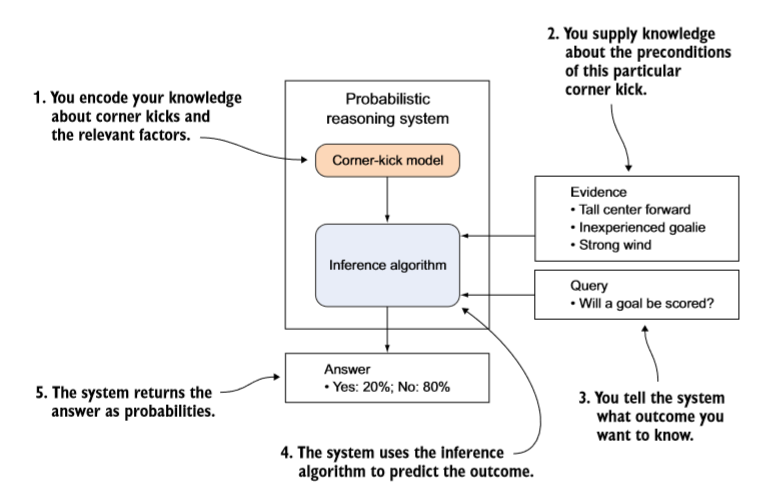
\includegraphics[width=\textwidth]{images/probabilistic_reasoning_system.PNG}
	\caption[General workflow example of a probabilistic reasoning system. Source: \cite{9781617292330}]{General workflow example of a probabilistic reasoning system}
	\label{fig:example_prs}
\end{figure}

\section{Lumen}

\subsection{Functionality}

compare to the plotting methods of PyMC3

\subsection{Requirements for a PPL}

possible criterium: variety of distributions that can be described?
\section{Comparing Different Probabilistic Programming Languages}

\begin{itemize}
     \item stan for python: https://pystan.readthedocs.io/en/latest/
    \item pymc3: https://docs.pymc.io/notebooks/getting\_started.html\#Case-study-2:-Coal-mining-disasters
    \item edward: http://edwardlib.org/getting-started
    \item pyro: http://pyro.ai/
\end{itemize}

\subsection{Stan for python}

transformed parameters are parameters which depend on hyperparameters.

\subsection{Pymc3}

PyMC3 is an open-source probabilistic programming framework for Python \cite{PyMC3_documentation}. Specification of Bayesian models in PyMC3 is done by encoding the prior, the sampling and the posterior distributions through three types of random variables: Stochastic, deterministic and observed stochastic ones. Stochastic random variables have values which are in part determined randomly, according to a chosen distribution. Commonly used probability distributions like Normal, Binomial etc. are available for this. Deterministic random variables, on the other hand, are not drawn from a distribution, but are calculated by fixed rules from other variables, for example by taking the sum of two variables. Lastly, there are the observed stochastic random variables which are similar to stochastic random variables, except that they get passed observed data as an argument, that should not be changed by any fitting algorithm.  This kind of random variable can be used to represent sampling distributions.
\\
PyMC3 mainly uses simulation techniques to draw inference on posterior distributions. It focuses especially on the No-U-Turn Sampler, a Markov Chain Monte Carlo algorithm, that relies on automated differentiation to get gradient information about continuous posterior distributions. PyMC3 also provides basic methods for plotting posterior distributions.
\\
The code piece  in \ref{fig:pymc3_example_code} shows a simple example of a Bayesian model, taken from the PyMC3 documentation at \cite{PyMC3_documentation}. There, the data X1, X2 and Y is used to fit a regression model. First, prior distributions for the model parameters are set up as stochastic random variables, then the regression model itself is specified by a deterministic random variable and lastly the sampling distribution is described by an observed stochastic random variable to which the observed outcome Y is given as a parameter. Finally, the posterior distribution is simulated by drawing 500 samples from it.

\begin{figure}
\begin{lstlisting}
import pymc3 as pm

basic_model = pm.Model()

with basic_model:
	# describe prior distributions of model parameters. Stochastic variables
	alpha = pm.Normal('alpha', mu=0, sd=10)
	beta = pm.Normal('beta', mu=0, sd=10, shape=2)
	sigma = pm.HalfNormal('sigma', sd=1)
	# specify model for the output parameter. Deterministic variable
	mu = alpha + beta[0]*X1 + beta[1]*X2
	# likelihood of the observations. Observed stochastic variable
	Y_obs = pm.Normal('Y_obs', mu=mu, sd=sigma, observed=Y)

# model fitting by using sampling strategies   
with basic_model:
# draw 500 posterior samples
trace = pm.sample(500)
pm.summary(trace)
\end{lstlisting}
\label{fig:pymc3_example_code}
\caption[Example code of a simple Bayesian model using PyMC3]{Example code of a simple Bayesian model using PyMC3}
\end{figure}

\subsection{Edward}

\subsection{Pyro}

\subsection{Choose the PPL for the task at hand}

\section{Practical implementation}
\section{Fallbeispiele}

\listoffigures
        
\section{Literatur}

\bibliography{Literatur.bib}
\bibliographystyle{ieeetr}


\end{document}